
Die Stromrechnung österreichischer Haushalte setzt sich aus drei strukturell unterschiedlichen Komponenten zusammen: 1) dem Energiepreis, 2) den Netzentgelten sowie 3) Steuern und Abgaben. Diese Unterscheidung ist für das Verständnis von INNOnet grundlegend, weil nur ein Teil davon durch regulatorische Tarifinstrumente adressierbar ist.

Der \textit{Energiepreis} umfasst die Beschaffung und den Vertrieb elektrischer Energie. Dieser Markt ist in Österreich seit der Liberalisierung Ende der 1990er-Jahre wettbewerblich organisiert: Kundinnen und Kunden wählen ihren Stromlieferanten frei und können bei Bedarf wechseln. Die Preise entstehen am Großhandelsmarkt und werden durch Angebot und Nachfrage bestimmt \parencite{econtrolSystemnutzungsentgelte}. Damit Haushalte möglichst alle relevanten Informationen zentral abrufen können, wurde in der App die Möglichkeit geschaffen, den individuellen Vertrag aus mehreren Anbietern auszuwählen und zu implementieren, sodass neben Netzentgelten auch Energietarife angezeigt werden.

Die \textit{Netzentgelte} vergüten nicht die Energie selbst, sondern deren Transport von der Erzeugungsanlage über Übertragungs- und Verteilnetze bis zur Steckdose. Da jeder Haushalt an ein physisch vorgegebenes regionales Verteilnetz angeschlossen ist, existiert für diesen Teil kein Wettbewerb. Die Netzentgelte werden deshalb nicht am Markt, sondern von der Regulierungsbehörde E-Control im Rahmen der Systemnutzungsentgelte-Verordnung festgesetzt \parencite{econtrolSystemnutzungsentgelte}. In Österreich machen Netzkosten je nach Tarif und Verbrauch typischerweise rund 30 bis 45\,\% der Gesamtstromrechnung aus \parencite{acerAnnualReport2022}.

Den dritten Teil bilden \textit{Steuern, Abgaben und Umlagen}: die Elektrizitätsabgabe \parencite{elabgg}, der Erneuerbaren-Förderbeitrag nach dem Erneuerbaren-Ausbau-Förderungsgesetz \parencite{eafg2021} sowie die Mehrwertsteuer. Diese Bestandteile sind gesetzlich fixiert und durch keinen Anbieterwechsel zu umgehen. Im Rahmen des INNOnet-Feldexperiments bleiben diese staatlichen Abgaben vollkommen unverändert.


\subsection{Aufgaben der Netzbetreiber}

Verteilnetzbetreiber (\textit{Distribution Network Operators}, DNOs) sind für den Transport elektrischer Energie auf den unteren Spannungsebenen zuständig -- von der Umspannstation bis zum Hausanschluss. Zu ihren Kernaufgaben gehören Planung, Betrieb, Wartung und Erneuerung der Netzinfrastruktur, der Anschluss neuer Verbraucher und Erzeuger sowie die Aufrechterhaltung der Versorgungssicherheit \parencite{elwog2010}.

Aus wirtschaftlicher Sicht sind Verteilnetze \textit{natürliche Monopole}: Ein zweites, paralleles Stromnetz für denselben Straßenzug zu errichten wäre volkswirtschaftlich sinnlos. Das Netz eines Betreibers weist hohe Fixkosten und sinkende Durchschnittskosten auf -- klassische Merkmale, die regulatorischen Eingriff rechtfertigen und erfordern \parencite{joskow2007, boiteux1960}. In Österreich setzt E-Control die zulässigen Erlöse der Netzbetreiber in mehrjährigen Regulierungsperioden fest und schafft dabei Anreize zur Kosteneffizienz \parencite{econtrolSystemnutzungsentgelte}.

Die Anforderungen an das Verteilnetz haben sich in den vergangenen Jahren grundlegend verändert. Historisch war das Netz darauf ausgelegt, Energie von wenigen großen Kraftwerken zu vielen kleinen Verbrauchern zu transportieren -- ein weitgehend unidirektionaler Fluss. Heute ist die Situation eine andere: Photovoltaikanlagen speisen Energie dezentral ein, Wärmepumpen und Elektrofahrzeuge erzeugen neue, teils gebündelte Lastspitzen. Ein Einfamilienhaus mit PV-Anlage, Wärmepumpe und Ladestation hat ein fundamental anderes Lastprofil als ein Haushalt aus den 1990er-Jahren \parencite{oesterreichsEnergie2023}.

Das eigentliche Netzproblem ist dabei nicht der Jahresverbrauch an sich, sondern die \textit{Gleichzeitigkeit}: Wenn viele Haushalte in einem Quartier ihre Wärmepumpen gleichzeitig hochregeln oder ihre Fahrzeuge gemeinsam nach der Heimkehr laden, entsteht eine lokale Lastspitze, die das Verteilnetz an seine Kapazitätsgrenzen bringen kann. Netze müssen jedoch für diese Spitzen ausgebaut werden, auch wenn sie nur wenige Stunden pro Jahr auftreten \parencite{borenstein2016, simshauser2016}.


\subsection{Netzentgelte: Funktion und Grenzen des Status quo}

Netzentgelte finanzieren die gesamte Infrastruktur des Verteilnetzes: Kabel, Transformatoren, Schaltanlagen, Zähler sowie Entstörungs-, Wartungs- und Erneuerungsbetrieb. Es handelt sich dabei im Wesentlichen um \textit{Fixkosten}: Die Infrastruktur muss bereitstehen, unabhängig davon, wie viel Energie gerade transportiert wird \parencite{borenstein2016}.

\begin{figure}
    \centering
    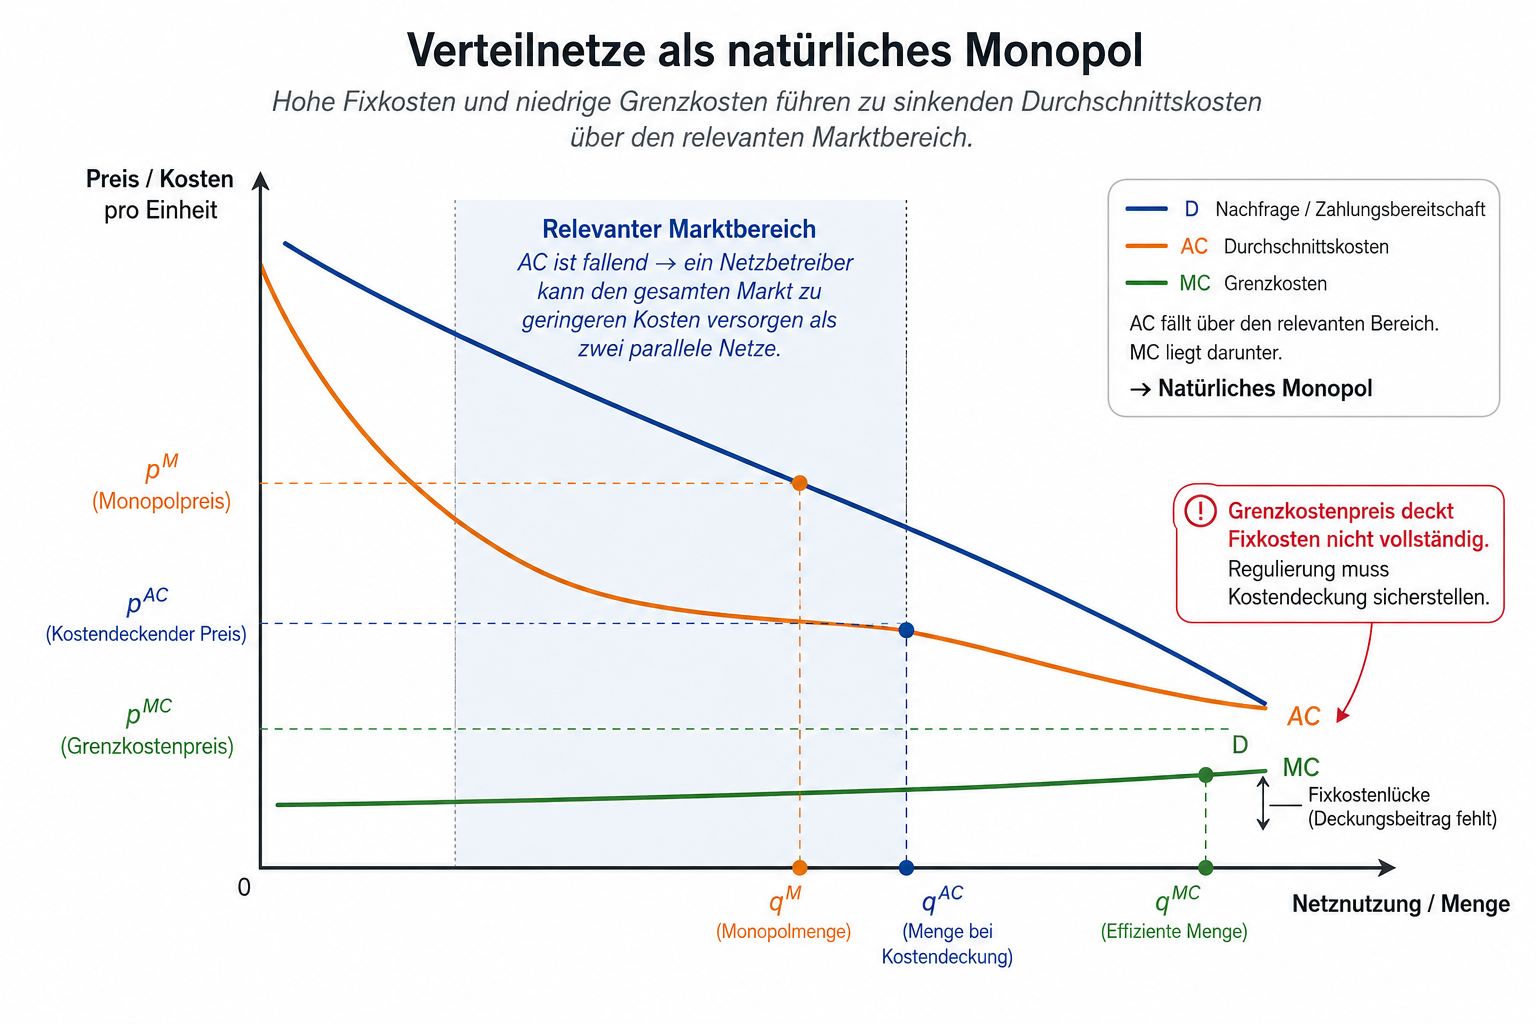
\includegraphics[width=1\linewidth]{paper/figures/Theory.png}
    \caption{Schematische Einordnung klassischer und lastabhängiger Netzentgelte.}
    \label{fig:theory_network_tariffs}
\end{figure}

Wie in weiten Teilen Europas setzt sich das klassische Netzentgelt in Österreich aus einem Arbeitspreis (pro kWh), einem Leistungspreis (pro kW Anschlussleistung oder Jahreshöchstlast) sowie fixen Bereitstellungsentgelten zusammen \parencite{econtrolSystemnutzungsentgelte}.
Der Arbeitspreis ist dabei zeitlich uniform: Es ist egal, ob ein Haushalt seine Waschmaschine um 7 Uhr morgens oder um 22 Uhr betreibt, ob er sein Elektrofahrzeug am Sonntagmittag oder am Montagabend lädt – der Netzpreis ist immer derselbe.

Aus ökonomischer Sicht ist das aus mehreren Gründen problematisch. Einerseits entstehen die relevanten Kosten eines Netzes maßgeblich durch Spitzenlasten, nicht durch den Durchschnittsverbrauch. Wenn die Kosten durch Spitzen bestimmt werden, sollte das Preissignal genau diese Spitzen adressieren. Dieses Prinzip ist in der ökonomischen Theorie als \textit{Peak-Load Pricing} bekannt \parencite{boiteux1960, williamson1966}. Andererseits honoriert ein einheitlicher Arbeitspreis weder das frühere Laden des Elektroautos noch den späteren Betrieb der Wärmepumpe, weshalb er keinen Anreiz zur zeitlichen Verschiebung des Verbrauchs gibt. Damit bleibt ein potenzieller Effizienzgewinn ungenutzt.



Die Regulierungsbehörden auf europäischer Ebene haben dieses Problem erkannt. Der \textit{Council of European Energy Regulators} (CEER) hat in seinen Berichten zu Distribution Network Tariffs darauf hingewiesen, dass zeitvariable oder lastabhängige Tarifsignale besser geeignet wären, die tatsächliche Netzbelastung abzubilden -- insbesondere angesichts der wachsenden Verbreitung steuerbarer Lasten \parencite{ceerDistributionTariffs2020, schittekatte2021}.

\textit{Dynamische Netzentgelte} sind ein Instrument, das diesen Zusammenhang aufgreift: Indem Netzentgelte zu Stunden höherer Netzbelastung höher und zu Stunden geringer Belastung niedriger angesetzt werden, erhalten Haushalte ein Preissignal, das eine zeitliche Verschiebung des Verbrauchs anreizen kann. Theoretisch können damit Lastspitzen abgeflacht, Netzausbau verringert und Systemkosten gesenkt werden. Ob und in welchem Ausmaß Haushalte auf solche Signale reagieren, ist hingegen eine empirische Frage, zu der die Literatur bislang heterogene Befunde liefert \parencite{faruquiSergici2010, newshamBowker2010}.


Dynamische Netzentgelte klingen in der Theorie plausibel. Die entscheidende Frage ist, was in der Praxis passiert: Reagieren Haushalte tatsächlich auf zeitvariable Netzsignale -- und wenn ja, wie stark, bei welchen Verbrauchern und unter welchen Bedingungen?

Diese Frage ist keineswegs trivial. Die finanziellen Anreize aus Netzentgelten sind im Verhältnis zum gesamten Haushaltsstrombudget gering. Die Tarifsignale sind oft komplex und im Alltag konkurrieren viele andere Faktoren mit dem Ziel der Verbrauchsverschiebung. Starke Verhaltenseffekte sind daher nicht selbstverständlich. Umso wichtiger ist es, mit einem sorgfältigen Studiendesign zu messen, was tatsächlich geschieht, statt die Wirkung regulatorischer Tarifinnovationen nur theoretisch herzuleiten.

Hier setzt das INNOnet-Projekt an, um diese empirische Forschungslücke für den österreichischen Kontext zu schließen. Untersucht wird, inwiefern Haushaltskunden ihren Stromverbrauch als Reaktion auf dynamische Netzentgelte anpassen, wenn die Tarifkomplexität durch eine bereitgestellte App reduziert wird. Der folgende Abschnitt beschreibt das zugrundeliegende experimentelle Tarifdesign sowie die technische Umsetzung der Informationsbereitstellung.
